\section{Searching for Stable Equilibria}\label{sec:equilibria}

In direct correspondence with common game theory language, it is possible to define basic relationships between the strategies.
Each organism's strategy $w$ encodes the probabilities of what actions it will take across its states.  A strategy is `pure' if these probabilities encode certainty of taking a single action per state otherwise it is `mixed'. Any mixed strategy can be decomposed into a linear combination of pure strategies. And any set of pure strategies defines a span of mixed strategies which can be linearly composed of them.
%The set of pure strategies which could feature in a linear decomposition of a mixed strategy is defined as the `support' of the mixed strategy.

If we define an `equilibrium' as being the condition where all the $\mathbf{M}_{P^*}^w$ population matrices remain constant - and an `equilibrium point' being defined by those matrices.
Then it is necessarily the case that an equilibrium leads to a condition where all the strategies that are significantly present in the population are steadily growing by the same growth-rate in steady-state. For if any organisms of a strategy existed in the population with a lesser steady-state growth-rate then it would proportionally die out, or if any organisms of a strategy existed with a greater steady-state growth-rate then it would lead the others to proportionately die out.

We further define the equilibrium as being `stable' in a similar way to Maynard Smith \cite{maynard, maynard2, weibull}, specifically if it cannot be disturbed from equilibrium by the presence of a small incorporation-of (or `invaded by') any possible `mutant' strategy. We note that this is at-least the case where no `mutant' strategy has a greater steady-state growth-rate in the context of the population.

In the next section \ref{appendix5} there is a demonstration that for any stable equilibrium established with a population of mixed strategies that it is possible to establish the same equilibrium point without the mixed strategies at all.
Informally the reasoning is that: because any mixed strategy is a stochastic mix of pure strategies then it can only perform as well as the best of them. And when it performs equal to the best then they must all perform equally. And in this case there is a combination of the pure strategies which have the same state-action profile $P^*$ as the mixed strategy; the same profile which defines the population matrices and thus the equilibrium point itself.
From these considerations it is thus unnecessary to consider mixed strategies in the search for stable equilibria because every stable equilibria can be established by combinations of pure strategies alone (although there may be zero or multiple such stable equilibria between them).

In our mathematics we assume that all population vectors grow exponentially under stable equilibrium with a common growth-rate equal to a maximum real non-negative eigenvalue (which may be one), and in proportions to a corresponding population matrix eigenvector.
This is a simplifying assumption and there exist possible population matrices where this assumption would be violated (specifically in the context of defective matrices), and in this context, other mathematics would need to be used to assert our conclusions.

\section{That any stable equilibrium point can always be rendered among pure strategies}\label{appendix5}
We consider a strategy's being \textit{replaceable} by other strategies if there exists a possible replacement of one's organisms for the others' in a population such as would not disturb the stable equilibrium point. The equilibrium point is defined by constant matrices $\mathbf{M}_{P^*}^w$, which is preserved at least when $P^*$ remains unchanged.
%Thus a strategy is replaceable at least when it can be replaced by organisms of other strategies such as not to change $P^*$.
If there is a stable equilibrium, each strategy $w$ has population in proportion to an eigenvector $\mathbf{n}^w$ with components $n^w_s$, thus its contribution to $P^*$ (per its definition) is:
$$P_{s,a}w_{a,s} \propto n^w_sw_{a,s}$$
The strategy is replaceable if there is a combination of other strategy's organisms to give this same contribution.

\begin{Definition}\label{def1}
A strategy $\bar{w}$ is \textbf{replaceable at stable equilibrium} by a set of other strategies $W$, if all strategies $w\in W$ are in equilibrium and thus have population matrices with the same maximal real eigenvalue and there exists non-negative corresponding eigenvectors $n^w_s$ and non-negative coefficients $d^w$ such that:
$$\forall a,s~~~~~~~~~~~ n^{\bar{w}}_s\bar{w}_{a,s} = \sum_{w\in W}d^wn^w_sw_{a,s} $$
\end{Definition}

Thus replaceability is a specific relationship between the eigenvectors of different strategy matrices and the weights of the strategies themself (which in turn determine those matrices).
Replaceability has an intuitive transitive property:

\begin{Definition}[Transitive Property of replaceability]\label{def3}
If organisms of strategy $A$ are replaceable by organisms of a set of strategies $B$, and if each of the organisms in the set of strategies in $B$ are replaceable by those of a set of strategies $C$, then organisms of strategy $A$ are also replaceable by those of set of strategies $C$.
\end{Definition}

In light of this we demonstrate that all mixed strategies are replaceable by pure strategies, by showing that every mixed strategy can be iteratively replaced by other strategies that are more `extreme':

\begin{Definition}\label{def2}
A strategy $w$ is \textbf{extreme} with respect to an action $a\in A_{s}$, if $w_{a,s}$ equals zero or one.\\A strategy $w$ is more \textbf{extreme} than another strategy $\bar{w}$ if $w$ is extreme with regards to more actions than $\bar{w}$ is.
\end{Definition}

To make our demonstration we first show that any specific mixed strategy can be decomposed into a linear combination of two strategies more extreme than it, and then we show that the mixed strategy is also replaceable by those two more extreme strategies.

\begin{Lemma}\label{lemma:part1}
Any mixed strategy $\bar{w}$ in stable equilibrium is replaceable by strategies which are more extreme.
\end{Lemma}
\begin{proof}
A mixed strategy $\bar{w}$ is (by definition of mixed) not extreme with regards to some action $\bar{a}\in A_{\bar{s}}$, then we consider two other similar strategies $w^1$ and $w^2$ that are otherwise the same except with re-weighted actions about the $\bar{s}$ state, such as to make them extreme in regards to action $\bar{a}$, ie. that $w^1_{\bar{a},\bar{s}}=1$ and $w^2_{\bar{a},\bar{s}}=0$.
$$ \mathbf{M}_{P^*}^{\bar{w}} = \bar{w}_{\bar{a},\bar{s}}\mathbf{M}_{P^*}^{w^1} + \left(\sum_{a\in A_{\bar{s}}\setminus \{\bar{a}\}} \bar{w}_{a,\bar{s}}\right)\mathbf{M}_{P^*}^{w^2} $$
$$\text{where}\qquad \forall a\in A_{\bar{s}}\setminus \{\bar{a}\},\qquad  w^1_{a,\bar{s}}=0 \quad\text{and}\quad w^2_{a,\bar{s}} = \frac{\bar{w}_{a,\bar{s}}}{\sum_{\hat{a}\in A_{\bar{s}}\setminus \{\bar{a}\}} \bar{w}_{\hat{a},\bar{s}}} $$
We note that if $\bar{w}$ is extreme with regards to any other action $a^*$ then the two other strategies $w^1$ and $w^2$ also extreme with regards to action $a^*$.
Thus any mixed strategy can be considered as a linear combination of two other strategies more extreme than it, all that remains to do is to show that this linear combination is also a replaceable combination aswell.\\
If we consider $\alpha = \bar{w}_{\bar{a},\bar{s}}$ then $\mathbf{M}_{P^*}^{\bar{w}} = \alpha\mathbf{M}_{P^*}^{w^1} + (1-\alpha)\mathbf{M}_{P^*}^{w^2} = \mathbf{M}(\alpha)$ and Theorems \ref{th:2} and \ref{th:3} apply.
Theorem \ref{th:2} informs us that the equilibrium growth rate (the spectral radius of the matrices) of strategies $w^1$ to $\bar{w}$ to $w^2$ is either monotonically increasing or decreasing or otherwise constant.
If it is monotonically increasing/decreasing then either $w^1$ or $w^2$ will have a greater equilibrium growth rate than $\bar{w}$, thus $\bar{w}$ is not part of stable equilibrium creating contradiction; thus $w^1$,$w^2$ and $\bar{w}$ must have the same growth rate.\\
Consequently Theorem \ref{th:3} informs us that the change in eigenvectors are linear, hence $\mathbf{n}^{\bar{w}} = \alpha \mathbf{n}^{w^1} + (1-\alpha)\mathbf{n}^{w^2}$ and that $n^{\bar{w}}_{\bar{s}} = n^{w^1}_{\bar{s}} = n^{w^2}_{\bar{s}}$ and selecting $d^{w^1} = \alpha$ and $d^{w^2} = 1-\alpha$ consequently satisfies definition \ref{def1}.
\end{proof}


\begin{Theorem}\label{the_proof}
Every mixed strategy in stable equilibrium is replaceable by a set of pure strategies 
\end{Theorem}
\begin{proof}
By Lemma \ref{lemma:part1} any mixed strategy can be replaced by other strategies that are more extreme than it, and those strategies (if they are mixed) can then be replaced by strategies which are even more extreme, and so on.
Thus by the transitive property (definition \ref{def3}), every mixed strategy can be replaced by ever increasing sets of strategies which are more extreme, and thus replaced by strategies which are most extreme - ie. pure strategies.
\end{proof}


\section{Example Evolutionary Model}

In this section illustrate the potential complexity of our modeling approach by detailing a evolutionary model and applying our solving software to discover points of equilibrium and disequilibrium.
We consider an evolutionary model of the sexual selection of a deleterious allele with a heterozygous advantage in simplified organisms with differing levels of parental investment under sexual selection with variable sexual diamorphism and survival factors.

Our motivation extends from surprising observation that the polygyny threshold model (specifically that polygyny should be positiely associated with resource/wealth inequality) appears to be an incorect hypothesis in the context of the cross-cultural analysis of human societies. \cite{item_2631714}
One possible explanation for this failure \cite{item_2631714} extends from the distinction between rival and non-rival wealth inheritance and their relative evolutionary importance.
Particularly where rival wealth (such as time-investment/money/resources) has less evolutionary relevance in comparrison with non-rival wealth (such as 'good genes') we might expect that efforts to select and secure rival wealth should be evolutionarily unmotivated and polygyny would be more frequent, and vice versa.

In order to interrogate the feasibility of this evolutionary reasoning, we constructed a structured and sexually symmetric simplified population model between $4$ age states, particularly: Infant $I$ and Young $Y$ and two Adult states $A_1$ and $A_2$.
In this model, individuals in state $I$ grow to become $Y$ and then have the opportunity to accept/reject a random reproductive pairing, they will then consequently age to become $A_1$ or $A_2$ depending on if their pairing was mutually accepted or not, where they will consequently then be randomly paired again.
This relationship between states is shown in Figure \ref{fig:age_states1} which encodes a simplistic model of parental investment, as the more the $Y$ reject partners and advance to being $A_2$ they will be investing in fewer offspring over a longer period of time.
The model includes several parameters, particularly: the degree to which being raised by zero/one/two $A_2$ parents and/or having different allels affects the survival of the offspring, the likelihood of a female in the model surviving childbirth, and a general mutation rate.

\begin{figure}
\centering
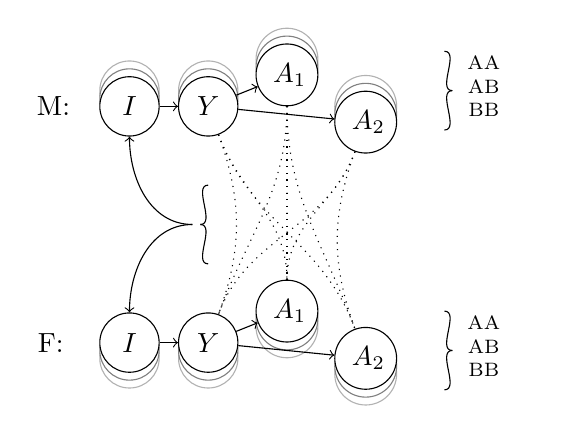
\begin{tikzpicture}


    \node [draw=gray!60, circle, text width=1em, align=center, fill=white] at (1,0.2) (IMab) {$I$};
    \node [draw=gray!60, circle, text width=1em, align=center, fill=white] at (2,0.2) (YMab) {$Y$};
    \node [draw=gray!60, circle, text width=1em, align=center, fill=white] at (3,0.6) (A1Mab) {$A_1$};
    \node [draw=gray!60, circle, text width=1em, align=center, fill=white] at (4,-0.0) (A2Mab) {$A_2$};
    \node [draw=gray, circle, text width=1em, align=center, fill=white] at (1,0.1) (IMab) {$I$};
    \node [draw=gray, circle, text width=1em, align=center, fill=white] at (2,0.1) (YMab) {$Y$};
    \node [draw=gray, circle, text width=1em, align=center, fill=white] at (3,0.5) (A1Mab) {$A_1$};
    \node [draw=gray, circle, text width=1em, align=center, fill=white] at (4,-0.1) (A2Mab) {$A_2$};
    
    \node [draw=gray!60, circle, text width=1em, align=center, fill=white] at (1,-3.2) (IFbb) {$I$};
    \node [draw=gray!60, circle, text width=1em, align=center, fill=white] at (2,-3.2) (YFbb) {$Y$};
    \node [draw=gray!60, circle, text width=1em, align=center, fill=white] at (3,-2.8) (A1Fbb) {$A_1$};
    \node [draw=gray!60, circle, text width=1em, align=center, fill=white] at (4,-3.4) (A2Fbb) {$A_2$};
    \node [draw=gray, circle, text width=1em, align=center, fill=white] at (1,-3.1) (IFab) {$I$};
    \node [draw=gray, circle, text width=1em, align=center, fill=white] at (2,-3.1) (YFab) {$Y$};
    \node [draw=gray, circle, text width=1em, align=center, fill=white] at (3,-2.7) (A1Fab) {$A_1$};
    \node [draw=gray, circle, text width=1em, align=center, fill=white] at (4,-3.3) (A2Fab) {$A_2$};



	\path [draw] (5.0,0.7) to[out=0,in=180] (5.1,0.2);
	\path [draw] (5.0,-0.3) to[out=0,in=180] (5.1,0.2);
    \node [text width=1cm,align=center] at (5.5,-0.05) (Maaabbb1) {\scriptsize BB};
    \node [text width=1cm,align=center] at (5.5,0.25) (Maaabbb2) {\scriptsize AB};
    \node [text width=1cm,align=center] at (5.5,0.55) (Maaabbb3) {\scriptsize AA};
	
	\path [draw] (5.0,0.7-3.3) to[out=0,in=180] (5.1,0.2-3.3);
	\path [draw] (5.0,-0.3-3.3) to[out=0,in=180] (5.1,0.2-3.3);
    \node [text width=1cm,align=center] at (5.5,-0.05-3.3) (Faaabbb1) {\scriptsize BB};
    \node [text width=1cm,align=center] at (5.5,0.25-3.3) (Faaabbb2) {\scriptsize AB};
    \node [text width=1cm,align=center] at (5.5,0.55-3.3) (Faaabbb3) {\scriptsize AA};
	


    \node [text width=1em, align=center] at (0,0) (M) {M:};
    \node [draw, circle, text width=1em, align=center, fill=white] at (1,0) (IM) {$I$};
    \node [draw, circle, text width=1em, align=center, fill=white] at (2,0) (YM) {$Y$};
    \node [draw, circle, text width=1em, align=center, fill=white] at (3,0.4) (A1M) {$A_1$};
    \node [draw, circle, text width=1em, align=center, fill=white] at (4,-0.2) (A2M) {$A_2$};
    
    \node [text width=1em, align=center] at (0,-3.0) (F) {F:};
    \node [draw, circle, text width=1em, align=center, fill=white] at (1,-3.0) (IF) {$I$};
    \node [draw, circle, text width=1em, align=center, fill=white] at (2,-3.0) (YF) {$Y$};
    \node [draw, circle, text width=1em, align=center, fill=white] at (3,-2.6) (A1F) {$A_1$};
    \node [draw, circle, text width=1em, align=center, fill=white] at (4,-3.2) (A2F) {$A_2$};
    
    \path [->,draw] (IM) -- (YM);
    \path [->,draw] (YM) -- (A1M);
    \path [->,draw] (YM) -- (A2M);
    
    \path [->,draw] (IF) -- (YF);
    \path [->,draw] (YF) -- (A1F);
    \path [->,draw] (YF) -- (A2F);

	\path [<-, draw] (IM) to[out=270,in=180] (1.8,-1.5);
	\path [<-, draw] (IF) to[out=90,in=180]  (1.8,-1.5);
	
	\path [draw] (2,-1) to[out=180,in=0] (1.9,-1.5);
	\path [draw] (2,-2) to[out=180,in=0] (1.9,-1.5);


    \path [draw, dotted] (YM) to[out=290,in=70] (YF);
    \path [draw, dotted] (YM) to[out=290,in=90] (A1F);
    \path [draw, dotted] (YM) to[out=290,in=110] (A2F);
    \path [draw, dotted] (A1M) to[out=270,in=70] (YF);
    \path [draw, dotted] (A1M) to[out=270,in=90] (A1F);
    \path [draw, dotted] (A1M) to[out=270,in=110] (A2F);
    \path [draw, dotted] (A2M) to[out=250,in=70] (YF);
    \path [draw, dotted] (A2M) to[out=250,in=90] (A1F);
    \path [draw, dotted] (A2M) to[out=250,in=110] (A2F);
    
\end{tikzpicture}
\caption{A population graph showing vital rates between age states}\label{fig:age_states1}
\end{figure}

In this model the primary point of strategic consideration which pairings each of the $Y$ will accept depending on their genotype. As there are three $Y$ genotypes to be paired with three possible genotypes for the opposite sex states ($Y$,$A_1$,$A_2$) thus there are $54$ possible pairings across $Y$s that they may be presented with, and which they may accept/reject.
As any strategy of accept/rejection is valid, there are thus $2^{54}$ pure strategies in this evolutionary model.

We begin each simulation starting from a population mean midpoint mixed strategy where each choice has a $50\%$ probability, and iterate using the software to resolve points of equilibrium (where the software converges to a stable strategy) or points of disequilibrium (particularly indicated by cycling of strategies).
In the output from this software, we plot the proportion of $Y$ accepting a match across the parameters of the model.
The results are shown in figure \ref{fig:model_results} where we see that the greater the heterozygous advantage of the allele, and the less the cost of parental noninvestment the greater the proprortion of $Y$ accepting pairings, which is our proxy for sequential polyginy.
Within this model, there are a range of thresholds where different strategies dominate over others across the parameters of the simulation.
The software is open source available and faciliates interrogation of this model with and/or without other factors and complexities as desired.

\begin{figure}
\centering
\begin{tikzpicture}
	\begin{axis}[view={-45}{35},
		xlabel=$x$,
		ylabel=$y$,
		zlabel={Vital Rate},
		title=A Scatter Plot Example,
		colormap/cool]
	\addplot3[surf] file 
		{output_Y.dat};
	\end{axis}
\end{tikzpicture}
\caption{The results you are looking for}\label{fig:model_results}
\end{figure}



\section{Conclusion}\label{sec:conclusion}

In this paper we have described a game in the context of non-linear population models, and we have given an equilibrium theorem \ref{the_proof} proving that all equilibria in such games can be found and described by proportions of pure strategies. This theorem's primary utility is that it eliminates the complexity of needing to consider the space of mixed strategies in searching-for and characterising such points of interest.

The elements of the game are simply that there be organisms which move between states in response to the actions and interactions with others,
and the only implicit limitation on such a game is that organisms be sufficiently numerous for their population and their dynamics to be modelled continuously.
Because of this flexibility, it is difficult to understate the potential span of things that could be represented, and therefore the potential applicability of our theorem.
The primary limitation of our theorem is the assumption that equilibrium growth-rates are given by population matrix eigenvalues/vectors (ie. no defective matrices) and thus it is interesting to consider what (if any) populations of things might naturally be described by defective matrices in which our theorem might also fail to hold.



